\tikzset{every picture/.style={line width=0.75pt}} %set default line width to 0.75pt        

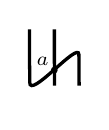
\begin{tikzpicture}[x=0.75pt,y=0.75pt,yscale=-1,xscale=1,scale=0.3]
%uncomment if require: \path (0,300); %set diagram left start at 0, and has height of 300

%Curve Lines [id:da8247822310570438] 
\draw[very thick]     (360.15,80) .. controls (359.9,154.08) and (360.77,137.11) .. (360.49,165.11) .. controls (360.2,193.11) and (439.06,98.26) .. (439.47,120.5) .. controls (439.88,142.74) and (439.26,139.92) .. (439.91,170.26) ;
%Straight Lines [id:da1404378491361742] 
\draw[very thick]   (400.11,80) -- (400.2,170.54) ;
%Shape: Circle [id:dp06914976647299276] 
\draw  [fill={rgb, 255:red, 0; green, 0; blue, 0 }  ,fill opacity=1 ] (396.4,145.42) .. controls (396.4,143.41) and (398.03,141.77) .. (400.05,141.77) .. controls (402.07,141.77) and (403.7,143.41) .. (403.7,145.42) .. controls (403.7,147.44) and (402.07,149.07) .. (400.05,149.07) .. controls (398.03,149.07) and (396.4,147.44) .. (396.4,145.42) -- cycle ;

% Text Node
\draw (366.8,120.37) node [anchor=north west][inner sep=0.75pt]  {${\scriptstyle a}$};


\end{tikzpicture}
